\documentclass{beamer}
%%% ========== Package setup ==========
\usepackage{xeCJK}      % Chinese words package
\usepackage{fontspec}   % Word fonts package
\usepackage{listings}   % Wrap Figure or table package
\usepackage{wrapfig}    % Multicolumn package
\usepackage{multicol}   % Multicolumn package
\usepackage{pdflscape}  % Landscpae package

%%% ========== Slide setting ==========
%% Slide theme setup
\usetheme{CambridgeUS}
\usecolortheme{wolverine}

%% Setup chinese words encoder
\XeTeXlinebreaklocale "zh"
\XeTeXlinebreakskip = 0pt plus 1pt

%% More word fonts
\setmainfont{Times New Roman}
\renewcommand{\familydefault}{\rmdefault}
\setCJKmainfont{標楷體}

% Setting for figure and table numbering
\setbeamertemplate{caption}[numbered]

%%% ========== Title setup ==========
\date{April 11, 2022}
\title{Meeting}
\author{Po Hsun Wu}

%%% ========== Document ==========
\begin{document}
\maketitle

\section{Progress report}

\begin{frame}
    \frametitle{\secname}

    \begin{itemize}
        \item Target function:
              $$f(x)=x^2$$
        \item Database:
              \begin{itemize}
                  \item $x=\{0,1,...,9\}$ adding noise with normal distribution($\mu=0, \sigma=0.2$).
                  \item 100 random data for each point(total of 1,000 data).
                  \item Train for 1000 times.
              \end{itemize}
    \end{itemize}
\end{frame}

\section{Result}

\begin{frame}
    \frametitle{\secname}
    \begin{itemize}
        \item Using two hidden layer, each layer with 50 neuros.
    \end{itemize}

    \begin{figure}
        \begin{multicols}{2}
            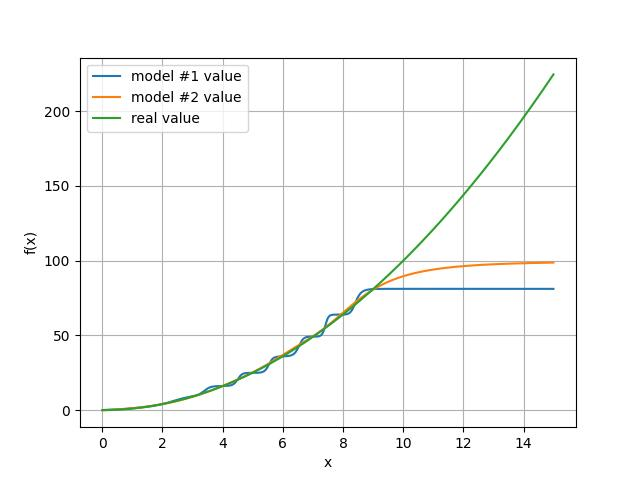
\includegraphics[width=2.2in]{Figs/Value_50_2.jpg}
            \caption{f(x) vs x}
            \columnbreak

            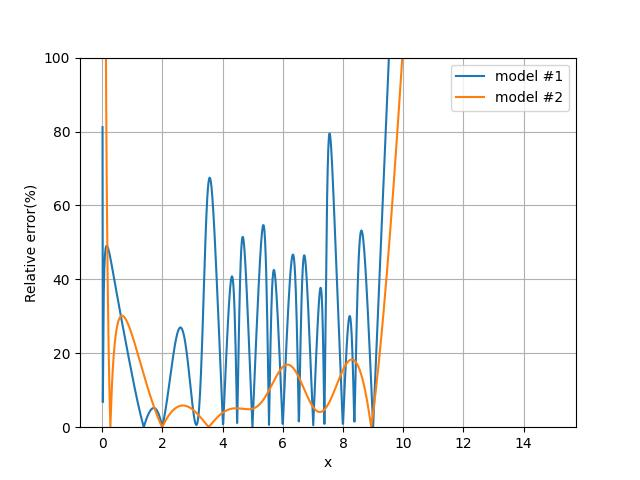
\includegraphics[width=2.2in]{Figs/Error_50_2.jpg}
            \caption{Relative error}
        \end{multicols}
    \end{figure}
\end{frame}

\begin{frame}
    \frametitle{\secname}
    \begin{itemize}
        \item Using three hidden layer, each layer with 50 neuros.
    \end{itemize}

    \begin{figure}
        \begin{multicols}{2}
            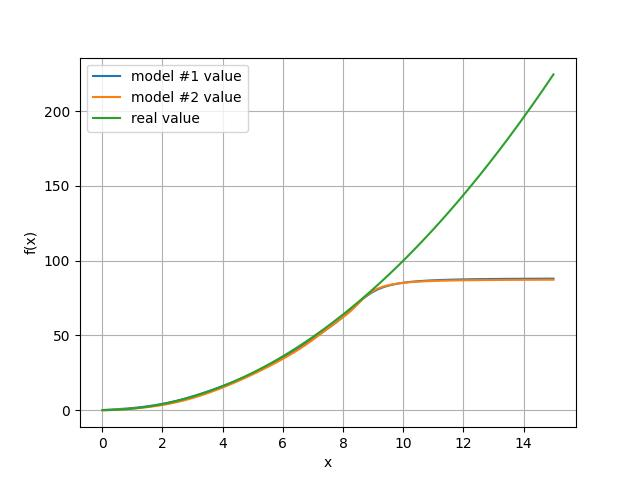
\includegraphics[width=2.2in]{Figs/Value_50_3.jpg}
            \caption{f(x) vs x}
            \columnbreak

            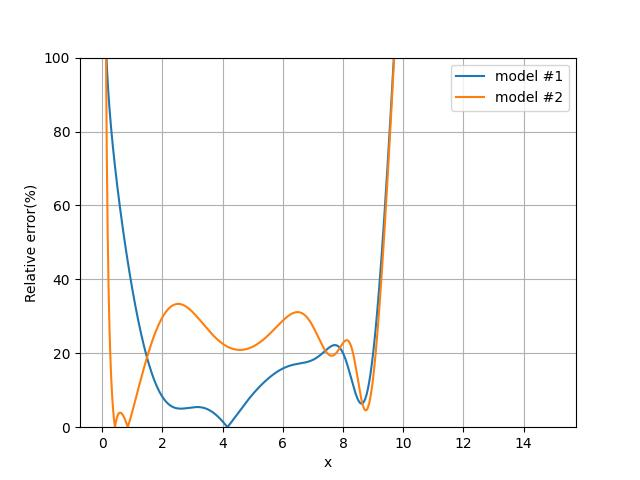
\includegraphics[width=2.2in]{Figs/Error_50_3.jpg}
            \caption{Relative error}
        \end{multicols}
    \end{figure}
\end{frame}

\begin{frame}
    \frametitle{\secname}
    \begin{itemize}
        \item Compare between 2 hidden layers and 3 hidden layers.
    \end{itemize}

    \begin{figure}
        \begin{multicols}{2}
            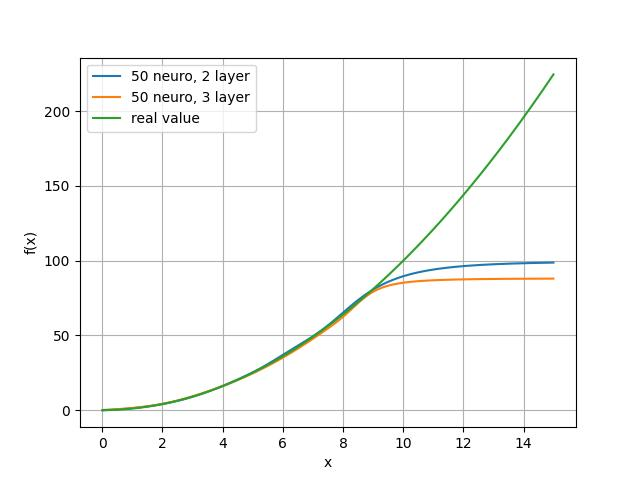
\includegraphics[width=2.2in]{Figs/Value_layer_compare.jpg}
            \caption{f(x) vs x}
            \columnbreak

            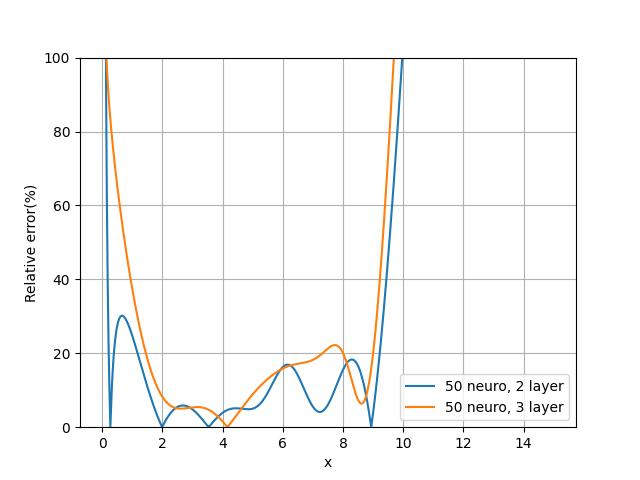
\includegraphics[width=2.2in]{Figs/Error_layer_compare.jpg}
            \caption{Relative error}
        \end{multicols}
    \end{figure}
\end{frame}

\begin{frame}
    \frametitle{\secname}
    \begin{itemize}
        \item Compare between 30 neuros and 50 neuros.
    \end{itemize}

    \begin{figure}
        \begin{multicols}{2}
            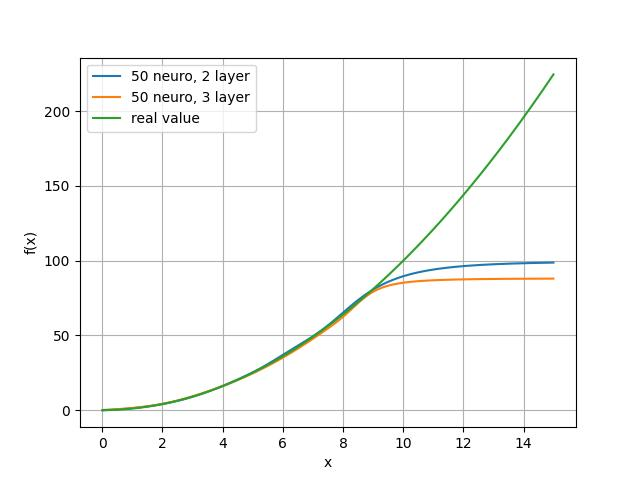
\includegraphics[width=2.2in]{Figs/Value_layer_compare.jpg}
            \caption{f(x) vs x}
            \columnbreak

            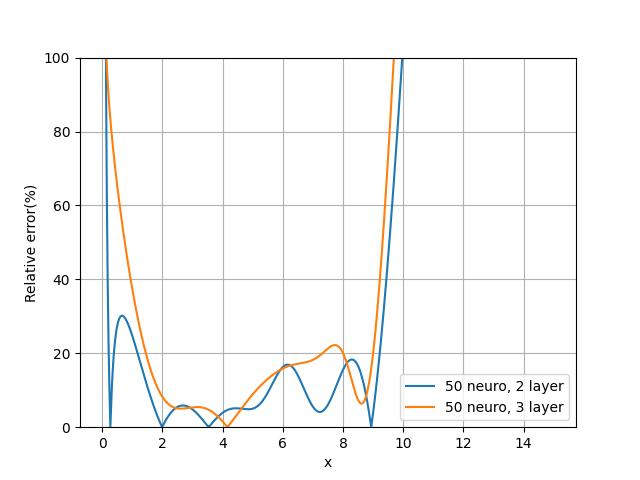
\includegraphics[width=2.2in]{Figs/Error_layer_compare.jpg}
            \caption{Relative error}
        \end{multicols}
    \end{figure}
\end{frame}

\begin{frame}
    \frametitle{\secname}
    \begin{itemize}
        \item Compare different learning rate.
    \end{itemize}

    \begin{figure}
        \begin{multicols}{2}
            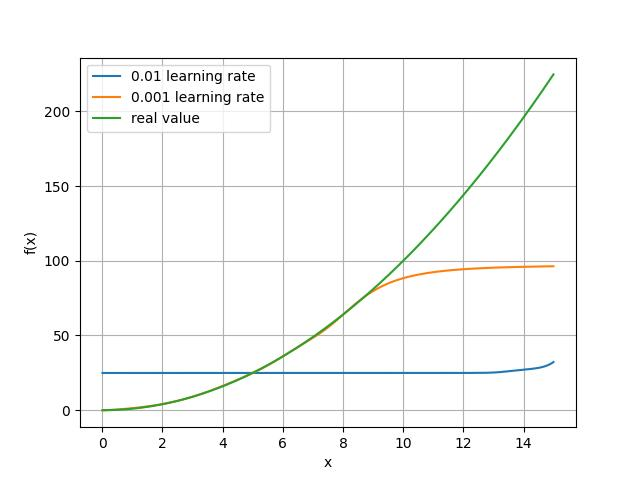
\includegraphics[width=2.2in]{Figs/Value_neuro_compare.jpg}
            \caption{f(x) vs x}
            \columnbreak

            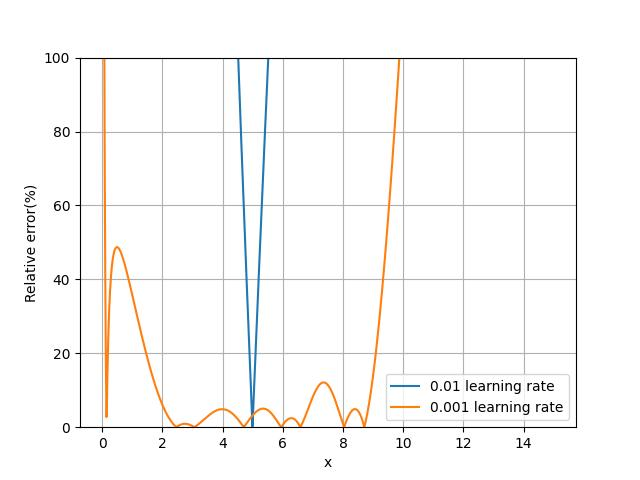
\includegraphics[width=2.2in]{Figs/Error_neuro_compare.jpg}
            \caption{Relative error}
        \end{multicols}
    \end{figure}
\end{frame}



\section{Source code}

\begin{landscape}
    \begin{frame}[fragile]

        \lstset{
            basicstyle=\fontsize{6.5}{6.5}\selectfont\setmainfont{Consolas},
            keywordstyle=\color{blue},
            numbers=left,
            numbersep=5pt
        }

        \begin{lstlisting}[language=Python]
import numpy as np
from tensorflow import keras

target_fun = lambda x: x * x

x = np.arange(0, 10, 1)
x = x.reshape((1, x.size))
x_ = np.repeat(x, 100, axis=0)
y = target_fun(x_).reshape((x_.size,))

init = initializer = keras.initializers.glorot_uniform()
model = keras.models.Sequential(
    [
        keras.layers.InputLayer(input_shape=(1,)),
        keras.layers.Dense(units=50, activation="sigmoid", kernel_initializer=init),
        keras.layers.Dense(units=50, activation="sigmoid", kernel_initializer=init),
        keras.layers.Dense(units=1, activation="linear", kernel_initializer=init),
    ]
)

noise = np.random.normal(0, 0.2, size=x_.shape)
x_noise = x_ + noise
x_noise = x_noise.reshape((x_noise.size,))

callback = [
    keras.callbacks.EarlyStopping(
        monitor="loss",
        patience=100,
        min_delta=0.001
    )
]
opt = keras.optimizers.SGD(
    learning_rate=0.001,
    momentum=0.005
)

model.compile(optimizer=opt, loss="MSE")
history = model.fit(
    x_noise, y,
    batch_size=10,
    epochs=1000,
    callbacks=callback,
    use_multiprocessing=True
)
        \end{lstlisting}

    \end{frame}
\end{landscape}

\end{document}